\documentclass[twocolumn,superscriptaddress]{revtex4-1}
\usepackage{graphicx}
\usepackage{epstopdf}
\usepackage{amsmath}
% \usepackage{hyperref}
\usepackage{booktabs}
\usepackage{color}
\usepackage{multirow}
\setlength{\tabcolsep}{10pt}

\begin{document}

\title{Increasing length scales in polydisperse hard spheres: the importance of multi-body correlations.} 

\author{Mathieu Leocmach}
\email{mathieu.leocmach@polytechnique.org}
\altaffiliation[Present address: ]{Laboratoire de Physique, CNRS UMR 5672, Ecole Normale Supérieure de Lyon, 46 allée d'Italie 69364 Lyon cedex 07, France.}
\author{John Russo}
\email{russoj@iis.u-tokyo.ac.jp}
\author{Hajime Tanaka}
\email{tanaka@iis.u-tokyo.ac.jp}
\affiliation{ {Institute of Industrial Science, University of Tokyo, 4-6-1 Komaba, Meguro-ku, Tokyo 153-8505, Japan} }

\date{Received \today}

\begin{abstract}
With numerical simulations of supercooled polydisperse hard spheres systems,
we show that the lengthscale associated with any two-point spatial correlation function
doesn't increase towards the glass transition. An increasing lengthscale is instead revealed
by considering multi-body correlation functions, such as correlators of orientational order.
We also reveal that the stability against crystallization with increasing polydispersity
is due to an increasing population of icosahedral arrangements of particles, competing with bond-orientationally
oriented regions which instead promote crystallization.

\end{abstract}

\maketitle

\section{Introduction}

Amorphous materials have been of prime importance in our technology for millennia, from antique glass works to the case of the last fashionable phone made of metallic glass. One of the new frontier of the amorphous technology is in the design of amorphous drugs~\cite{Petit2006,Grzybowska2012}, better absorbed by our metabolism with less side effects, that would be stable at room temperature. The main obstacle is our lack of basic understanding of the physics of the glass transition, without any operative consensus despite half a century of intensive research~\citep{cavagna2009supercooled,BerthierR}.

When cooled below its freezing temperature while avoiding crystallisation, a liquid becomes supercooled. Upon further cooling, the dynamics slows down by many orders of magnitude leading to a material that is mechanically a solid without long range positional order, thus called amorphous. It is now known that the dynamics inside a supercooled liquid is heterogeneous, with a length scale that grow when approaching the glass transitionn~\citep{yamamoto1998,Donati1999a} (see~\citep{BerthierR} for a review). The lengthscale defined by the dynamical heterogeneity is not static (one-time spatial correlation) but dynamic (two-time spatial correlation).

The existence of a static (structural) length that would grow and accompany the dynamic heterogeneities is still not clear in the general case. However, in a class of system that includes polydisperse hard spheres, we have shown~\cite{tanaka} that some medium range bond orientational order reminiscent of the crystal exists in the supercooled liquid and grows toward the glass transition in the same way as the dynamical heterogeneity. The presence in glassy materials of structures locally reminiscent of crystals has been confirmed recently in amorphous silicon~\cite{Treacy2012} and in a metallic glass~\cite{Hwang2012}.

Bond order-related parameters and correlation lengths are intrinsically multi-body quantities. However, the only exact (in the mean-field, infinite dimension approximation) theory of the glass transition, the Mode-coupling theory (MCT), takes as input only two-body quantities. Modern spin-glass-type theories of the structural glass transition~\cite{lubchenko2007,Biroli2008,Parisi2010} are building on the MCT (considered as a mean-field limit), while not taking explicitly into account multi-body correlations.

In the present paper, we will use the now well studied polydisperse hard sphere system where we know how to extract meaningful multi-body correlations and look for a two-body quantity that would show the same behaviour as the bond order. We will show that the two-body part of the free energy and the two-body part of the structural entropy are unable to capture medium range bond ordered regions or to yield length meaningful from the point of view of the glass transition. We thus confirm the medium range crystalline order scenario and test its robustness against increasing polydispersity.


\section{Methods}
We run isothermal-isobaric NpT Monte Carlo simulations of $N=4000$ polydisperse hard spheres.
The diameters ($\sigma$) follow a Gaussian distribution $P(\sigma)=\exp{\left[-(\sigma-\sigma_0)^2/2\,s^2\right]}/\sqrt{2\pi} s$,
with polydispersity index $\delta=s/\sigma_0$. In the following we fix the unit of length as $\sigma_0=1$.

Our aim is to compare the behaviour of both two-point quantities and multi-body quantities with increasing pressure.
Due to the hard-sphere interaction, entropy is the only contribution to the system free energy.
All two-pair correlation quantities are thus derived from the two-body excess entropy~\cite{Nettleton1958,Mountain1971},
defined as
\begin{equation}
s_2=-\frac{\rho}{2}\int dr\left[g(r)\log(g(r))-g(r)+1\right]
\end{equation}
In principle, $s_2$ can be calculated separately for each particle $i$ in the system. In practice, this requires short time averages to compute the pair correlation function of each particle, $g_i(r)$\cite{tanaka}. We instead construct an approximate but instantaneous $s_2(i)$ using the global $g(r)$
\begin{equation}
s_2(i) = -\frac{\rho}{2}\sum_j \left[g(r_{ij})\log(g(r_{ij}))-g(r_{ij})+1\right].
\end{equation}
This quantity is in very good agreement with the short time average procedure when the averaging time is comparable to the $\beta$ relaxation ; however the results can be very different if the averaging time becomes comparable or longer than the $\alpha$ relaxation, like in Ref.~\cite{tanaka}.

Alternatively, one can compute directly the free-energy of each configuration by
considering the free volume, defined as the volume ($v(i)$) in which each sphere can freely
move while holding all the other spheres fixed. It has been shown~\cite{Aste2004} that this free
volume is simply related to the pair free-energy ($f_2$) by the following relation
\begin{equation}
f_2=\sum_i f_2(i)=-k_BT\sum_i \log(v(i)/\lambda)
\end{equation}
where $\lambda$ is the thermal wavelength. To compute the free volume we follow previous
studies: first the Voronoi-diagram for each configuration is computed, and the polyhedron
surrounding each particle is determined. The free volume of particle $i$ is then
computed by shifting normally all the faces of the corresponding polyhedron by $\sigma(i)/2$
towards particle $i$, and computing the new volume. This procedure is conducted indipendentely
for each particle and for each configuration.



To study multi-body correlations we use the local bond-order analysis introduced by
\citet{steinhardt}, first applied to study crystal nucleation by
Frenkel and co-workers~\cite{auer}. 
The $\ell$-fold symmetry of a neighbourhood around each particle $i$ is characterised by a $(2\ell+1)$ dimensional complex vector ($\mathbf{q}_l$) as $q_{\ell m}(i)=\frac{1}{N_b(i)}\sum_{j=1}^{N_b(i)} Y_{\ell m}(\mathbf{\hat{r}_{ij}})$, where
$\ell$ is a free integer parameter, and $m$ is an integer
that runs from $m=-\ell$ to $m=\ell$. The functions $Y_{\ell m}$ are the spherical harmonics
and $\mathbf{\hat{r}_{ij}}$ is the vector from particle $i$ to particle $j$.
The sum goes over all neighbouring particles $N_b(i)$ of particle $i$. Usually 
$N_b(i)$ is defined by all particles within a cutoff distance, but in an inhomogeneous system
the cutoff distance would have to change according to the local density. Instead we 
fix $N_b(i)=12$ which is the number of nearest neighbours in icosahedra and close packed crystals (like \textsc{hcp} and \textsc{fcc})
which are known to be the only relevant structures for hard spheres.

In the analysis, one uses the rotational invariants defined as:
\begin{align}
	q_\ell =& \sqrt{\frac{4\pi}{2l+1} \sum_{m=-\ell}^{\ell} |q_{\ell m}|^2 }, \label{eq:ql}\\
	w_\ell =& \sum_{m_1+m_2+m_3=0} 
			\left( \begin{array}{ccc}
				\ell & \ell & \ell \\
				m_1 & m_2 & m_3 
			\end{array} \right)
			q_{\ell m_1} q_{\ell m_2} q_{\ell m_3}. \label{eq:wl}
\end{align}
where the term in brackets in Eq.~(\ref{eq:wl}) is the Wigner 3-j symbol.
In particular both crystalline and icosahedral neighbourhood have high $q_6$ (strong 6-fold symmetry), with the highest values for the later. To detect specifically icosahedral order one prefers $w_6$, whose minimum value is obtained only by a perfect icosahedron. To detect specifically crystal-like order, one should use their extendability: two neighbouring crystal-like neighbourhood should have similar orientation, thus similar vectorial $\mathbf{q}_6$.

The scalar product $(\mathbf{q}_6(i)/|\mathbf{q}_6(i)|)\cdot(\mathbf{q}_6(j)/|\mathbf{q}_6(j)|)$ quantifies this similarity. If it exceeds $0.7$ between
two neighbours, they are deemed \emph{connected}. We then identify a particle as crystalline if it is connected with at least $7$ neighbours~\cite{auer}. In a more continuous way, summing the contribution of all the bonds of a given particle, we define the ``crystallinity''~\cite{russo_hs}
\begin{equation}\label{eqn:crystallinity}
 \text{C}(i)=\sum_{j=0}^{N_b(i)}\frac{\mathbf{q}_6(i)\cdot\mathbf{q}_6(j)}{|\mathbf{q}_6(i)|\,|\mathbf{q}_6(j)|}.
\end{equation}

Alternatively, one can coarse-grain $\mathbf{q}_\ell$ over the neighbours~\cite{lechner}
\begin{equation}
	Q_{\ell m}(i) = \frac{1}{N(i)+1}\left( q_{\ell m}(i) +  \sum_{j=0}^{N(i)} q_{\ell m}(j)\right), 
	\label{eq:Qlm}
\end{equation}
and use the resulting invariant $Q_6$ as an indication of crystallinity.

We note that both $\text{C}$ and $Q_6$ are no direct indicator for the presence of crystals, but rather measures for a tendency to promote crystallisation.

\section{Results}

\begin{figure}
 \centering
 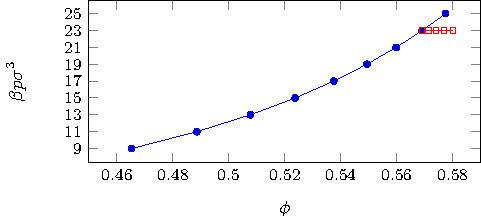
\includegraphics{fig_eos}
 \caption{\textbf{Simulated state points.} The circles (blue curve) represent the equation of state for polydispersity $\delta=7\%$. The squares (red curve) instead are simulation points at the same pressure ($\beta p\sigma^3=23$) but at different polydispersities $\delta$: from low to high volume fraction they correspond to $\delta=7\%,9\%,11\%,13\%,15\%$ respectively.}
 \label{fig:eos}
\end{figure}


Fig.~\ref{fig:eos} shows the equation of state for the simulated state points. In particular
we consider two data-sets. The first one (black circles in the figure) corresponds to
simulations at a constant polydispersity of $\delta=7\%$. For each state point we run $8$ independent
simulation runs and extract configurations for the calculation of correlation lengths.
The second data set (red cicles in the figure) are instead isobaric simulation (at $\beta p\sigma^3=23$)
with increasing polydispersity, $\delta=7\%,9\%,11\%,13\%,15\%$. These state points are used to study
the mechanism by which crystallization is suppressed upon increase of polydispersity, unveiling the
role played by icosahedral arrangement of particles.

\subsection{Order parameter distribution and mobility}

\begin{figure}
	\centering
	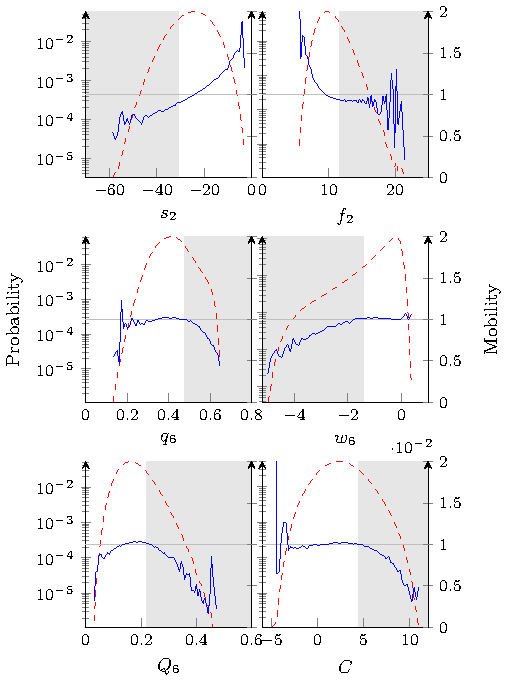
\includegraphics{fig_distrib}
	\caption{\textbf{Probability distribution} (red dash) \textbf{and mobility} (blue continuous) function of various order parameter at $\beta p\sigma^3=25$ and for a time difference corresponding to the $\alpha$-relaxation. Mobility is in unit of mean-square displacement. The limit of the shaded area is at one standard deviation from the mean value of the order parameter in the direction of ordering.}
	\label{fig:distrib}
\end{figure}

We study systematically two-body ($s_2$, $f_2$) and multi-body ($q_6$, $w_6$, $Q_6$, $C$) scalar order parameter fields for our highest pressure ($\beta p\sigma^3=25$). Figure~\ref{fig:distrib} shows the probability distribution of these parameters, always skewed toward the ordered side (shaded in Fig.~\ref{fig:distrib}).

By plotting the probability distribution function for the metastable fluid on the $f_2$, $Q_6$ and $w_6$ axis we note the absence of any linear correlation between $f_2$ and both $Q_6$ and $w_6$. Since $Q_6$ identifies crystal-like bond-orientationally ordered regions, and $w_6$ locates icosahedral arrangements of particles, it is clear that high $f_2$ regions are not associated with any of these structures. We checked in the same way that $s_2$ is not correlated with multi-body parameters.

\begin{figure}
 \centering
 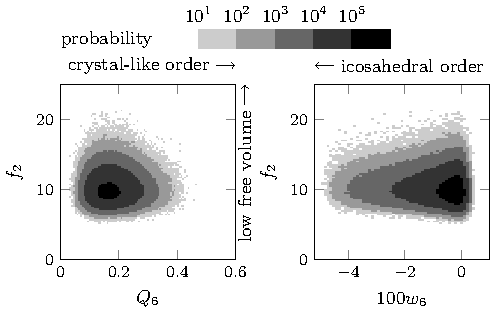
\includegraphics{fig_f2decoupling}
 \caption{\textbf{Correlation between two-body and multi-body parameters.} Probability distribution functions in the $f_2$,$Q_6$-map (top) and in the $f_2$,$w_6$-map (bottom) for a metastable fluid with polydispersity $\delta=7\%$ and pressure $\beta p\sigma^3=23$. The parameters are not correlated, even in extreme values.}
 \label{fig:f2decoupling}
\end{figure}

To study the correlation between any scalar order parameter $x$ and the displacement of the particles, we define the mobility 
\begin{equation}
	\Delta r^2(x=x_0, t) \equiv \left\langle \frac{
		\sum\limits_i{
			\left\|\mathbf{r}_i(t)-\mathbf{r}_i(0)\right\|^2 \delta(x(i)-x_0)
			}
	}{
		\sum\limits_i{\delta(x(i)-x_0)}
	}\right\rangle,
	\label{eq:mobility}
\end{equation}
shown in Fig.~\ref{fig:distrib} for a time difference corresponding to the $\alpha$-relaxation. Mobility always decreases with increasing order. The mobilities of bond-order quantities are flat in the disordered regions and decrease when approaching the perfect structure (i.e. icosahedron for $w_6$, crystal cell for $Q_6$ or $C$). By contrast, the mobility of two-body order parameters tends to decrease strongly in the disordered region and less in the ordered region (it is almost flat at high $f_2$). We conclude that two-body quantities describe well the faster dynamics of some disordered particles whereas multi-body quantities describe better the slowing down accompanying good local ordering.

Both fast and sow particles are a priori important to describe dynamic heterogeneities, thus we cannot discard the relevance of either two-body or multi-body parameters based on this analysis.

\subsection{Length-scales}
\begin{figure}
	\centering
	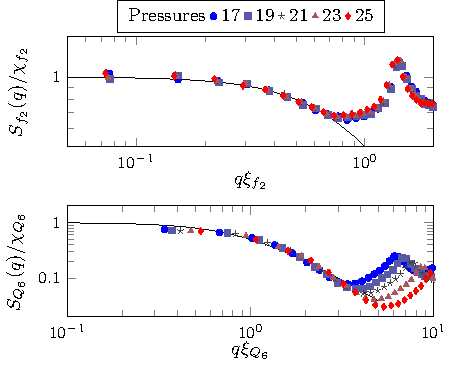
\includegraphics{fig_structurefactor}
	\caption{\textbf{Structure factors} collapse on the Ornstein-Zernike form for (top) $f_2$ and (bottom) $C$. Note how the former are almost similar across pressures.}
	\label{fig:structurefactor}
\end{figure}

\begin{figure}
	\centering
	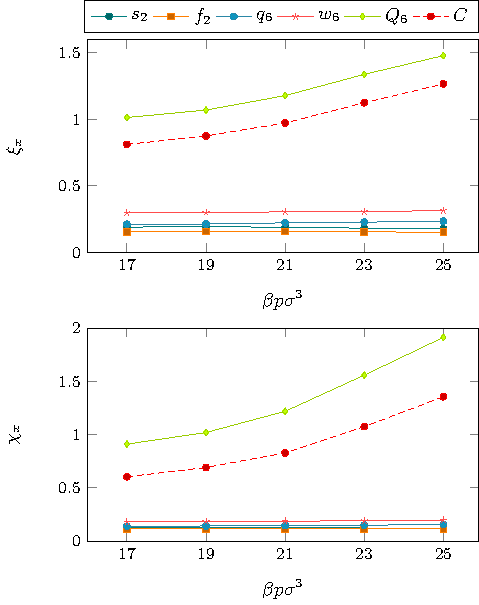
\includegraphics{fig_lengths}
	\caption{\textbf{Correlation length} extracted for two-body and multi-body scalar order parameters, function of the pressure. Only multi-body correlation lengths are increasing (only slightly for $\xi_{w_6}$), while the lenghscale associated with the two-body quantities is constant.}
	\label{fig:Fourierlengths}
\end{figure}

\begin{figure}
	\centering
	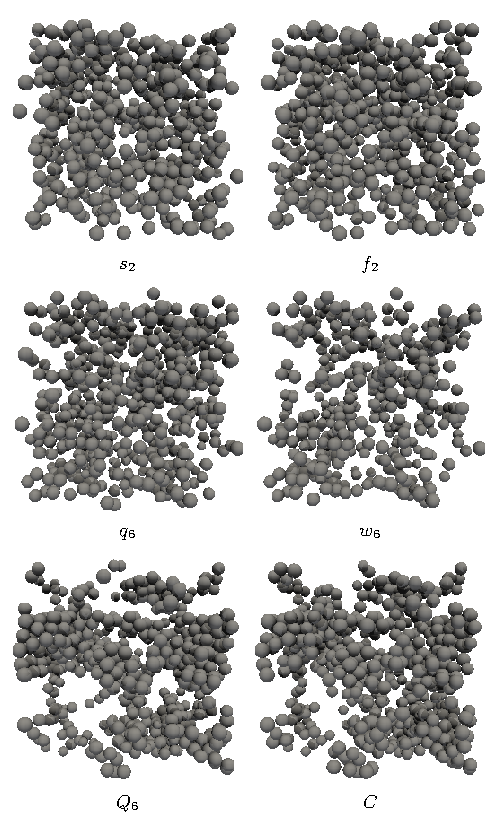
\includegraphics{fig_3D}
	\caption{\textbf{Visualisation of the ordered regions} defined by the various order parameters. All pictures correspond to the same configuration at $\beta p\sigma^3=23$ and $\delta=7\%$. Only $Q_6$, $C$ and (much smaller) $w_6$ show meaningful fluctuations.}
	\label{fig:3D}
\end{figure}

We have shown previously~\cite{tanaka,kawasaki,mathieu_icosahedra,russo_gcm,russo_hs} how to compute the correlation length of the crystal-like order in real space using its tensorial nature. However, to allow the comparison with the scalar two-body parameters, we use here a single method for all parameters in Fourier space.

For any scalar order parameter field $x$ increasing with order, we define the threshold 
\begin{equation}
x^* \equiv \langle x\rangle + \sqrt{\langle x^2\rangle - \langle x\rangle^2},
\label{eq:xstar}
\end{equation}
at one standard deviation above the average value. We then compute a four-point structure factor keeping only the ordered particles ($x>x^*$). The thresholds are indicated on Fig.~\ref{fig:distrib}. Formally we define a function $\omega(i) = \Theta [x(i) - x^*]$, where $\Theta(x)$ is Heaviside’s step function, and a four-point structure factor
\begin{equation}
	S_x(q) = N^{-1}(\left\langle \Omega(\mathbf{q}) \Omega(-\mathbf{q}) \right\rangle - | \left\langle \Omega(\mathbf{q}) \right\rangle^2 |),   
	\label{eq:StrutureFactor}
\end{equation}
where $\Omega(\mathbf{q})$ is the Fourier transform of $\omega(i)$: 
\begin{equation}
	\Omega(\mathbf{q}) = \sum_i \omega(i)\exp(-\imath \mathbf{q}\cdot\mathbf{r}_i).  
\end{equation}
The case of order parameters decreasing toward ordering (i.e. $s_2$, $w_6$) is trivially obtained by changing the sign.

As shown in Fig.~\ref{fig:structurefactor}, the small wave-vector behaviour of $S_x(q)$ is well described by the asymptotic Ornstein-Zernike function in Fourier space:
\begin{equation}
	S_x(q\rightarrow 0) \approx \frac{\chi_x}{1+\xi_x^2 q^2},
	\label{eq:OZ_Fourier}
\end{equation}
where $\xi_x$ is the correlation length and $\chi_x$ the susceptibility. In general, an independent determination of $\chi_x$ is crucial for the fit~\cite{Flenner2011}. However here we deal with correlation lengths much smaller than the simulation box and both $\xi_x$ and $\chi_x$ can be reliably estimated from a two parameter fit of $S_x(q)$.

The dependence on the pressure of the resulting correlation lengths is shown on Fig.~\ref{fig:Fourierlengths}. Most of the order parameters produce constant lengthscales, including the two-body quantities and $q_6$, $w_6$ that are sensible to icosahedral order. The only growing lengths are extracted from measures of local crystal-like order, i.e. $Q_6$ and $C$. This result is confirmed by visualizing (see Fig.~\ref{fig:3D}) the ordered particles defined by each order parameter. Only $Q_6$ and $C$ show clustering of the ordered particles on medium range.

We checked that similar results are obtained in real space for scalar two-body and tensorial multi-body (sensible only to crystal-like structures) order parameters. We also checked that the constance of the length of two-body parameters was not affected by the definition of the threshold $x^*$, either smaller, larger or equal to the average value $\langle x\rangle$ (the absolute value of the length is affected by this definition, but not the pressure dependence).

The study of correlation lengths have shown that by increasing pressure, the range of
crystal-like bond-orientational order increases, and as shown in Ref.~\cite{tanaka,mathieu_icosahedra}
driving the slowing down of the system. Bond-orientational order corresponds to
orientationally ordered regions which spontaneously form in the metastable phase.
$f_2$ is instead decoupled from the relevant structures involved in the transition, as
shown in Fig.~\ref{fig:f2decoupling}.





\subsection{Competition between icosahedral arrangements and crystalline arrangements}

\begin{figure}
 \centering
 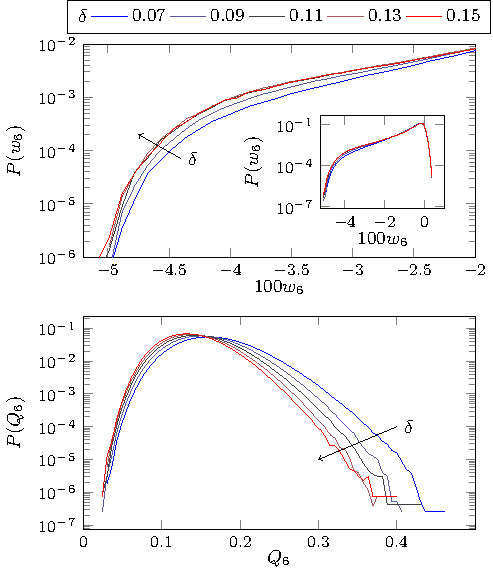
\includegraphics{fig_polydistrib}
 \caption{\textbf{Effect of polydispersity} on local structures at constant pressure ($\beta p\sigma^3=23$). \textbf{top} detail of the distribution of $w_6$ (full distribution in inset) showing a small increase in the icosahedra population saturating around $10\%$. \textbf{bottom} distribution of $Q_6$ showing a marked decrease in the crystallinity.}
 \label{fig:polydispersity}
\end{figure}

We will now focus on the state point at $\beta p\sigma^3=23$ at different polydispersities to
study the mechanism by which polydispersity disfavours the crystallization transition.

In Fig.~\ref{fig:polydispersity} we show the probability distributions for the order
parameters $Q_6$ and $w_6$ and for different polydispersities. It is immediately
evident that, while bond-orientational order is rapidly suppressed with increasing
polydispersity (as shown in the suppressed signal at high $Q_6$, maybe saturating around $\delta=15\%$), particles in icosahedral
environments are not disfavoured by polydispersity. On the contrary the fraction of
icosahedral particles increases with polydispersity, and saturates at around $\delta=10\%$.

\begin{figure}
 \centering
 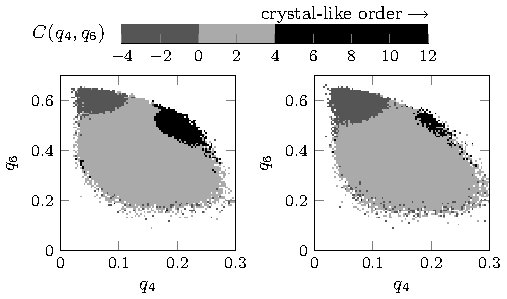
\includegraphics{fig_Cmaps}
 \caption{Average crystallinity order parameter projected in the $q_4$,$q_6$ space for the metastable fluid at $\beta p\sigma^3=23$ at $\delta=7\%$ (top) and $\delta=15\%$. Icosahedra appear in the top-left corner of each plot and perfect \textsc{fcc} crystals would be in the top-right corner.}
 \label{fig:Cmaps}
\end{figure}


Figure~\ref{fig:Cmaps} shows that the metastable fluid distribution presents both characteristic
structures: icosahedral environments with high $q_6$, low $q_4$ and negative $C$; crystal-like bond ordered regions with high values of
$q_4$, $q_6$ and $C$. The main difference between the low and
high polydispersity metastable states is the population of the crystal-like bond ordered regions.


\begin{figure}
 \centering
 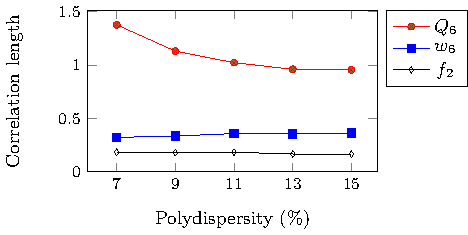
\includegraphics{fig_lengthpoly}
	\caption{\textbf{Polydispersity dependence of the correlation lengths} at $\beta p\sigma^3=23$. The dominant crystalline length decreases, the icosahedral length increases, however they plateau well before crossing. The two-body length shows no indication of becoming dominant with increasing $\delta$, even decreasing slightly.}
	\label{fig:lengthpoly}
\end{figure}

In the same way, the correlation length extracted from $Q_6$ decreases with increasing polydisersity, while the one extracted from $w_6$ increases (see Fig.~\ref{fig:lengthpoly}). However the two lengths are far from crossing and seem to saturate around $\delta=13-15\%$. The correlation length of $f_2$ is constant or even slightly decreasing with $\delta$, not at all taking over the multi-body lengths. Thus, in the range of polydispersity that we studied crystal-like bond order fluctuations seem to rule the system static (and probably dynamic) properties.


In the metastable fluid a competition between bond-ordered regions and icosahedral regions takes
place, with polydispersity favouring the latter. The nature of the competition can be seen
in two-dimensional maps of translational vs orientational order, i.e. $\phi,q_6$ maps.
As was shown in Ref.~\cite{russo_hs}, this plot is very useful in determining the region
of thermodynamic stability of each phase. The calculation is straightforward: for each
configuration, particles are identified as ``fluid'' and ``crystalline'' according to
the criteria described in the methods section. For each subset of particles, the
the average value of the volume fraction
$\phi$ is calculated as a function of the order parameter $q_6$. By looking at the
relative position of the two curves (the one for the fluid particles and the other for the crystalline particles)
the relative stability of the phases can be determined: at each volume fraction,
the stable phase is the one with the higher value of $q_6$. 

\begin{figure}
 \centering
 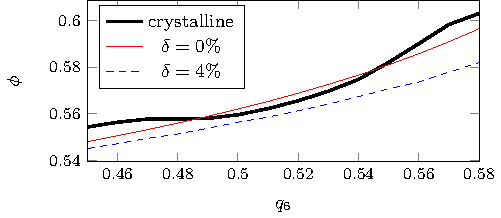
\includegraphics{fig_stability_map}
 \caption{Average $\phi$ as a function of $q_6$ for particles identified as fluid and crystalline. The continuous red curve represents fluid particles in a system at $\beta p\sigma^3=17$ and $\delta=0\%$, while dashed blue curve represents fluid particles at the same pressure but at $\delta=4\%$. The thick black curve represents instead solid particles (this curve is less sensitive to polydispersity and it is reported once).}
 \label{fig:stability_map}
\end{figure}

In Fig.~\ref{fig:stability_map}
we compare the curves at $\beta p\sigma^3=17$ and at different polydispersities:
at $0\%$ (monodisperse system, black circles) and at $4\%$ (red squares). The curve for the
crystalline particles is similar at the two considered polydispersities and is reported once
as the dashed line. First we consider he monodisperse case. As shown in the figure,
at low volume fraction, the stable phase is the fluid phase. But at $\phi\cong 55.8\%$ a crossover
occurs and the crystal phase gains stability. This stability is again lost at $\phi\cong 58\%$
because at high $q_6$ values the liquid branch is composed entirely of icosahedral particles.
At polydispersity $\delta=4\%$ the crystalline branch is always metastable to the fluid one.
This is due to an increase in $q_6$ of the fluid branch at high $\phi$, which shifts ``below'' the
crystalline curve. The behaviour of the fluid curve is due to an increased population of
icosahedral particles, which dominate the fluid branch for $q_6\gtrsim 0.5$. The fact that
the crystalline phase loses its metastability window is immediately evident in simulations,
as at this pressure it is not possible to crystallize simulations at $\delta=4\%$, while the
monodisperse simulations have a small nucleation time.

We have thus provided direct evidence that icosahedral particles are responsible for the suppression
of crystallization in polydisperse hard spheres.

\paragraph*{\bf Author Contributions}
M.L., J.R. and H.T. conceived the research, discussed and wrote the manuscript ; J.R. performed the simulations, M.L. and J.R. performed the analysis. M.L. and J.R. contributed equally to this work.


\bibliographystyle{apsrev4-1}
\bibliography{biblio}

\end{document}
